% Holonomía y curvatura
% Compilar con: pdflatex holonomy_curvature.tex
\documentclass[tikz,border=10pt]{standalone}
\usepackage{tikz}
\usepackage{amsmath}
\usepackage{xcolor}
\definecolor{gdlblue}{RGB}{41, 98, 168}
\definecolor{gdlred}{RGB}{191, 49, 49}
\definecolor{gdlgreen}{RGB}{30, 130, 76}
\definecolor{gdlorange}{RGB}{217, 130, 30}
\definecolor{gdlpurple}{RGB}{118, 56, 138}
\definecolor{gdlgray}{RGB}{140, 140, 140}
\definecolor{gdlyellow}{RGB}{190, 140, 10}
\usetikzlibrary{arrows.meta, decorations.pathmorphing, calc}

\begin{document}
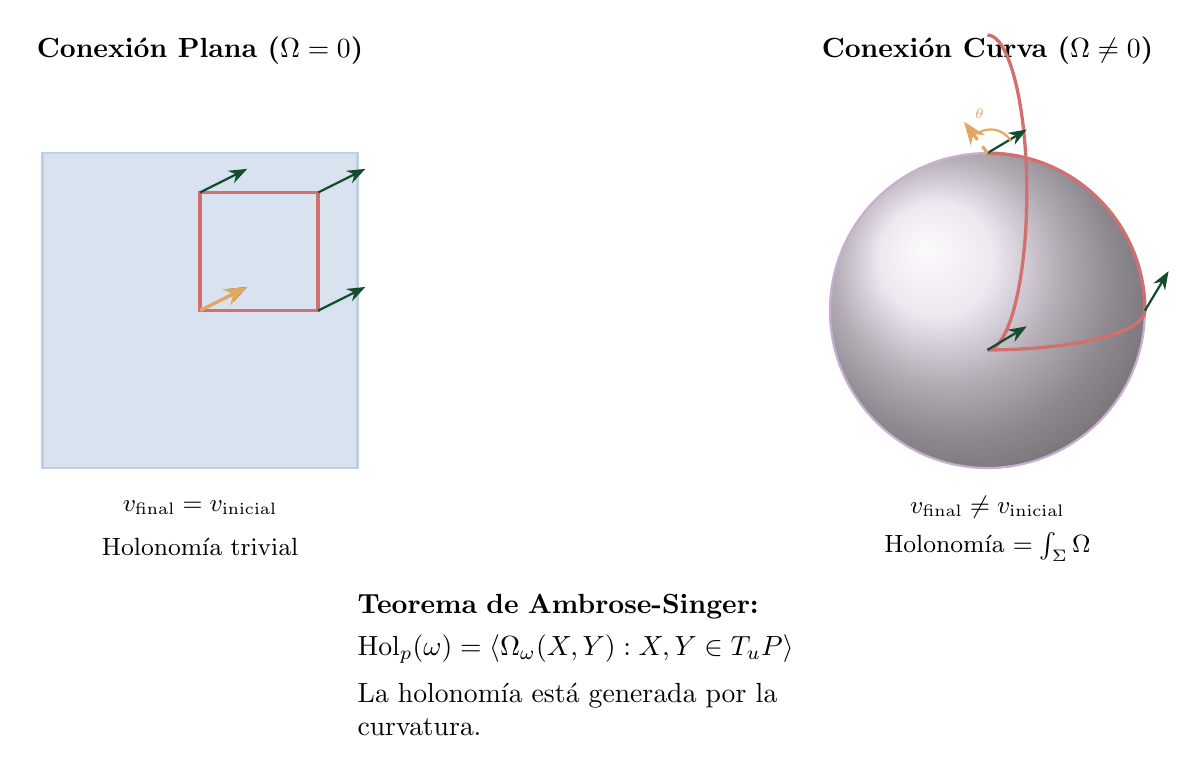
\begin{tikzpicture}[>=Stealth]

% === Conexión plana (sin holonomía) ===
\begin{scope}[shift={(-5, 0)}]
    \node[above, font=\bfseries] at (0, 3) {Conexión Plana ($\Omega = 0$)};

    % Plano
    \fill[gdlblue!18] (-2, -2) rectangle (2, 2);
    \draw[thick, gdlblue!30] (-2, -2) rectangle (2, 2);

    % Lazo
    \draw[very thick, gdlred!70] (0, 0) -- (1.5, 0) -- (1.5, 1.5) -- (0, 1.5) -- cycle;

    % Vectores transportados (todos paralelos)
    \draw[->, thick, gdlgreen!60!black] (0, 0) -- (0.6, 0.3);
    \draw[->, thick, gdlgreen!60!black] (1.5, 0) -- (2.1, 0.3);
    \draw[->, thick, gdlgreen!60!black] (1.5, 1.5) -- (2.1, 1.8);
    \draw[->, thick, gdlgreen!60!black] (0, 1.5) -- (0.6, 1.8);

    % Vector final = inicial
    \draw[->, very thick, gdlorange!70] (0, 0) -- (0.6, 0.3);
    \node[font=\small] at (0, -2.5) {$v_{\text{final}} = v_{\text{inicial}}$};
    \node[font=\small] at (0, -3) {Holonomía trivial};
\end{scope}

% === Conexión curva (con holonomía) ===
\begin{scope}[shift={(5, 0)}]
    \node[above, font=\bfseries] at (0, 3) {Conexión Curva ($\Omega \neq 0$)};

    % Esfera parcial
    \shade[ball color=gdlpurple!20, opacity=0.8] (0, 0) circle (2cm);
    \draw[thick, gdlpurple!40] (0, 0) circle (2cm);

    % Lazo en la esfera
    \draw[very thick, gdlred!70]
        (0, 2) arc (90:0:2cm) arc (0:-90:2cm and 0.5cm) arc (-90:90:0.5cm and 2cm);

    % Vectores transportados (rotan)
    \draw[->, thick, gdlgreen!60!black] (0, 2) -- (0.5, 2.3);
    \draw[->, thick, gdlgreen!60!black] (2, 0) -- (2.3, 0.5);
    \draw[->, thick, gdlgreen!60!black] (0, -0.5) -- (0.5, -0.2);

    % Vector final ≠ inicial
    \draw[->, very thick, gdlorange!70, dashed] (0, 2) -- (-0.3, 2.4);

    \node[font=\small] at (0, -2.5) {$v_{\text{final}} \neq v_{\text{inicial}}$};
    \node[font=\small] at (0, -3) {Holonomía $= \int_\Sigma \Omega$};

    % Ángulo de rotación
    \draw[thick, gdlorange!70] (0.3, 2.15) arc (30:120:0.3cm);
    \node[gdlorange!70, font=\tiny] at (-0.1, 2.5) {$\theta$};
\end{scope}

% === Fórmula central ===
\node[font=\normalsize, text width=6cm] at (0, -4.5) {
    \textbf{Teorema de Ambrose-Singer:}\\[0.3em]
    $\mathrm{Hol}_p(\omega) = \left\langle \Omega_\omega(X, Y) : X, Y \in T_u P \right\rangle$\\[0.5em]
    La holonomía está generada por la curvatura.
};

\end{tikzpicture}
\end{document}
